\documentclass[a4paper,11pt]{article}
\usepackage[T1]{fontenc}
\usepackage[utf8]{inputenc}
\usepackage[english]{babel}
\usepackage{amsmath,amssymb,mathtools}
\usepackage[margin=2.2cm]{geometry}
\usepackage{xcolor,tikz}
\usepackage[most]{tcolorbox}
\setlength{\parindent}{0pt}
\setlength{\parskip}{4pt}
\allowdisplaybreaks
\providecommand{\explainmode}{0}
\newif\ifexplain
\ifnum\explainmode=1 \explaintrue\fi
\newcommand{\aufgabe}[1]{\section*{#1}}
\newcommand{\angabe}[1]{\textit{#1}\par\smallskip}
\newcommand{\teil}[1]{\subsection*{#1}}
\newcommand{\why}[1]{\text{\small\color{black!65}#1}}
\newtcolorbox{erklbox}{colback=blue!4,colframe=blue!40,breakable,boxrule=0.5pt,title={Erklärung}}
\newcommand{\explain}[1]{\ifexplain\begin{erklbox}#1\end{erklbox}\fi}
\newcommand{\explainfig}[1]{\ifexplain\begin{center}#1\end{center}\fi}
\begin{document}
\begin{center}
{\Large Exercise sheet 7}\\
Linear Optimization (311.160), WS 2026/27\\
Raphael Bleier \qquad 16 November 2026
\end{center}
\explain{Dieses Blatt ist das Dualitätsblatt. Zuerst wird ein ganzes Tableau nach Bland's Rule durchpivotiert. Sechs degenerierte Schritte, die die Ecke gar nicht bewegen, und erst der letzte Schritt bringt den Zielfortschritt. Danach wird zu einem konkreten LP das duale Problem aufgestellt und an jeweils drei primalen und dualen Punkten die schwache Dualität nachgerechnet. Aufgabe 7.3 schließlich rekonstruiert aus dem Beweis des Strong-Duality-Theorems, warum ein optimales primales $x^*$ automatisch ein optimales duales $y^*$ mitliefert.}

\explain{Classroom task 7.1, nur als Lernzusatz, nicht Teil der Abgabe. System (1) bündelt drei Dinge: $Ax=b,\ x\ge 0$ heißt, dass $x_0$ primal zulässig ist, $A^T\tilde x\ge c$ heißt, dass $\tilde x_0$ dual zulässig ist, und $c^Tx_0\ge b^T\tilde x_0$ ist die umgekehrte Weak-Duality-Ungleichung. Die schwache Dualität (Theorem 3.3) liefert für jedes zulässige Paar $c^Tx\le b^T\tilde x$, insbesondere $c^Tx_0\le b^T\tilde x_0$. Zusammen mit $c^Tx_0\ge b^T\tilde x_0$ erzwingt das $c^Tx_0=b^T\tilde x_0$. Nach Corollary 3.4 ist damit $x_0$ optimal für das LP (und $\tilde x_0$ optimal für das duale). Antwort: $x_0$ ist eine Optimallösung des LPs, und $(x_0,\tilde x_0)$ ist ein Zertifikat dafür, weil primaler und dualer Zielfunktionswert übereinstimmen.}

\aufgabe{Exercise 7.1 (On the simplex method)}
\angabe{Consider the following initial simplex tableau:
\[
\begin{aligned}
z &= x_1 - 2x_2 - 2x_4\\
x_5 &= -\tfrac12 x_1 + \tfrac72 x_2 + 2x_3 - 4x_4\\
x_6 &= -\tfrac12 x_1 + x_2 + \tfrac12 x_3 - \tfrac12 x_4\\
x_7 &= 1 - x_1
\end{aligned}
\]
Use the simplex method to find the optimal solution by applying Bland's rule.}
\explain{Das Tableau ist ein Dictionary: links stehen die Basisvariablen $x_5,x_6,x_7$, rechts die Nichtbasisvariablen $x_1,\dots,x_4$. Die zweite und dritte Zeile sind im Original beide mit $x_5$ beschriftet; da die vierte $x_7$ heißt, behandle ich die dritte Zeile als $x_6$. Eine Basis darf keine Variable doppelt enthalten.}
\explain{Bland's Rule legt zwei Dinge fest, um Zyklen zu vermeiden: Als eintretende Variable nimmt man unter allen Nichtbasisvariablen mit positiven reduzierten Kosten die mit dem kleinsten Index; als austretende unter allen Zeilen mit minimalem Quotienten die mit dem kleinsten Basisindex. Die Startecke $(0,0,0,0,0,0,1)$ ist degeneriert, weil $x_5=x_6=0$ Basisvariablen sind. Deshalb sind die ersten Schritte degenerierte Pivots mit Schrittweite $0$: Die Ecke und $z$ bleiben stehen, nur die Basis wechselt. Genau dafür braucht es Bland's Rule.}
\explain{Vorzeichenkonvention für den Quotiententest: In der Zeile $x_i=\bar b_i-\sum_j \bar a_{ij}x_j$ steht vor $x_j$ der Koeffizient $-\bar a_{ij}$. Der Quotiententest rechnet mit $\bar a_{ij}$, also mit dem Negativen des hingeschriebenen Koeffizienten. Ein positiver hingeschriebener Koeffizient bedeutet $\bar a_{ij}<0$ und liefert keinen Quotienten.}

\teil{Initial dictionary}
The source labels both middle rows $x_5$. I interpret the second of these as $x_6$, so the three basic variables are distinct. All coefficients are unchanged.\par
The basis is $B=\{5,6,7\}$, the nonbasis $N=\{1,2,3,4\}$. Setting the nonbasic variables to zero gives the basic feasible solution $x=(0,0,0,0,0,0,1)^T$ with $z=0$. The reduced costs are the coefficients of the objective row:
\begin{align*}
\bar c_N &= (1,\,-2,\,0,\,-2) && \why{read off $z = x_1 - 2x_2 - 2x_4$}
\end{align*}

\teil{Pivot 1: $x_1$ enters, $x_5$ leaves}
The only positive reduced cost is $\bar c_1=1$, so $x_1$ enters. The column of $x_1$ has entries $\bar a = (\tfrac12,\tfrac12,1)^T$:
\begin{align*}
\tfrac{0}{1/2} &= 0 && \why{ratio in the $x_5$ row}\\
\tfrac{0}{1/2} &= 0 && \why{ratio in the $x_6$ row}\\
\tfrac{1}{1} &= 1 && \why{ratio in the $x_7$ row}
\end{align*}
The minimum is $0$, attained by both $x_5$ and $x_6$. Bland's rule picks the smaller index, so $x_5$ leaves. Solve the $x_5$ row for $x_1$:
\begin{align*}
x_5 &= -\tfrac12 x_1 + \tfrac72 x_2 + 2x_3 - 4x_4 && \why{row of $x_5$}\\
\tfrac12 x_1 &= -x_5 + \tfrac72 x_2 + 2x_3 - 4x_4 && \why{$|\,+\tfrac12 x_1 - x_5$}\\
x_1 &= -2x_5 + 7x_2 + 4x_3 - 8x_4 && \why{$|\,\cdot 2$}
\end{align*}
Substitute into the remaining rows:
\begin{align*}
x_6 &= -\tfrac12 x_1 + x_2 + \tfrac12 x_3 - \tfrac12 x_4 && \why{row of $x_6$}\\
&= -\tfrac12(-2x_5 + 7x_2 + 4x_3 - 8x_4) + x_2 + \tfrac12 x_3 - \tfrac12 x_4 && \why{substitute $x_1$}\\
&= x_5-\tfrac72x_2-2x_3+4x_4+x_2+\tfrac12x_3-\tfrac12x_4 && \why{distribute and multiply}\\
&= x_5 - \tfrac52 x_2 - \tfrac32 x_3 + \tfrac72 x_4 && \why{collect terms}\\
x_7 &= 1 - x_1 && \why{row of $x_7$}\\
&=1-(-2x_5+7x_2+4x_3-8x_4) && \why{substitute $x_1$}\\
&= 1 + 2x_5 - 7x_2 - 4x_3 + 8x_4 && \why{distribute the minus sign}\\
z &= x_1 - 2x_2 - 2x_4 && \why{objective row}\\
&= -2x_5 + 7x_2 + 4x_3 - 8x_4 - 2x_2 - 2x_4 && \why{substitute $x_1$}\\
&= -2x_5 + 5x_2 + 4x_3 - 10x_4 && \why{collect terms}
\end{align*}
\[
\begin{aligned}
z &= -2x_5 + 5x_2 + 4x_3 - 10x_4\\
x_1 &= -2x_5 + 7x_2 + 4x_3 - 8x_4\\
x_6 &= x_5 - \tfrac52 x_2 - \tfrac32 x_3 + \tfrac72 x_4\\
x_7 &= 1 + 2x_5 - 7x_2 - 4x_3 + 8x_4
\end{aligned}
\]
Now $B=\{1,6,7\}$, $N=\{2,3,4,5\}$, reduced costs $(5,4,-10,-2)$, and the basic solution is still $(0,0,0,0,0,0,1)^T$ with $z=0$.
\explain{Der Pivot ist degeneriert: Die Schrittweite ist $0$, $x_1$ kommt mit Wert $0$ in die Basis, $x_5$ verlässt sie mit Wert $0$. Die Ecke und $z$ ändern sich nicht. Die Basiswerte bestätigen das: $x_1=x_6=0$, $x_7=1$ wie vorher.}

\teil{Pivot 2: $x_2$ enters, $x_6$ leaves}
Reduced costs are $(5,4,-10,-2)$ for $(x_2,x_3,x_4,x_5)$. The positive ones are $x_2$ and $x_3$; Bland's rule picks the smaller index, so $x_2$ enters. Its column has $\bar a = (-7,\tfrac52,7)^T$:
\begin{align*}
\tfrac{0}{5/2} &= 0 && \why{ratio in the $x_6$ row}\\
\tfrac{1}{7} &= \tfrac17 && \why{ratio in the $x_7$ row}
\end{align*}
The minimum is $0$, so $x_6$ leaves. Solve the $x_6$ row for $x_2$:
\begin{align*}
x_6 &= x_5 - \tfrac52 x_2 - \tfrac32 x_3 + \tfrac72 x_4 && \why{row of $x_6$}\\
\tfrac52 x_2 &= x_5 - x_6 - \tfrac32 x_3 + \tfrac72 x_4 && \why{$|\,+\tfrac52 x_2 - x_6$}\\
x_2 &= \tfrac25 x_5 - \tfrac25 x_6 - \tfrac35 x_3 + \tfrac75 x_4 && \why{$|\,\cdot \tfrac25$}
\end{align*}
Substitute into the remaining rows:
\begin{align*}
x_1 &= -2x_5 + 7x_2 + 4x_3 - 8x_4 && \why{row of $x_1$}\\
&= -2x_5 + 7(\tfrac25 x_5 - \tfrac25 x_6 - \tfrac35 x_3 + \tfrac75 x_4) + 4x_3 - 8x_4 && \why{substitute $x_2$}\\
&= -2x_5+\tfrac{14}{5}x_5-\tfrac{14}{5}x_6-\tfrac{21}{5}x_3+\tfrac{49}{5}x_4+4x_3-8x_4 && \why{distribute and multiply}\\
&= \tfrac45 x_5 - \tfrac{14}{5} x_6 - \tfrac15 x_3 + \tfrac95 x_4 && \why{collect terms}\\
x_7 &= 1 + 2x_5 - 7x_2 - 4x_3 + 8x_4 && \why{row of $x_7$}\\
&=1+2x_5-7(\tfrac25x_5-\tfrac25x_6-\tfrac35x_3+\tfrac75x_4)-4x_3+8x_4 && \why{substitute $x_2$}\\
&=1+2x_5-\tfrac{14}{5}x_5+\tfrac{14}{5}x_6+\tfrac{21}{5}x_3-\tfrac{49}{5}x_4-4x_3+8x_4 && \why{distribute and multiply}\\
&= 1 - \tfrac45 x_5 + \tfrac{14}{5} x_6 + \tfrac15 x_3 - \tfrac95 x_4 && \why{collect terms}\\
z &= -2x_5 + 5x_2 + 4x_3 - 10x_4 && \why{objective row}\\
&= -2x_5 + 5(\tfrac25 x_5 - \tfrac25 x_6 - \tfrac35 x_3 + \tfrac75 x_4) + 4x_3 - 10x_4 && \why{substitute $x_2$}\\
&= -2x_5+2x_5-2x_6-3x_3+7x_4+4x_3-10x_4 && \why{distribute and multiply}\\
&= -2x_6 + x_3 - 3x_4 && \why{collect terms}
\end{align*}
\[
\begin{aligned}
z &= -2x_6 + x_3 - 3x_4\\
x_1 &= \tfrac45 x_5 - \tfrac{14}{5} x_6 - \tfrac15 x_3 + \tfrac95 x_4\\
x_2 &= \tfrac25 x_5 - \tfrac25 x_6 - \tfrac35 x_3 + \tfrac75 x_4\\
x_7 &= 1 - \tfrac45 x_5 + \tfrac{14}{5} x_6 + \tfrac15 x_3 - \tfrac95 x_4
\end{aligned}
\]
Now $B=\{1,2,7\}$, $N=\{3,4,5,6\}$, reduced costs $(1,-3,0,-2)$.

\explain{Hier wird die zweite Basiszeile nach $x_2$ aufgelöst. Beim Einsetzen müssen die Faktoren $7$ und $5$ jeweils die ganze Klammer multiplizieren. Auch dieser Schritt hat Länge null.}

\teil{Pivot 3: $x_3$ enters, $x_1$ leaves}
The only positive reduced cost is $\bar c_3=1$, so $x_3$ enters. Its column has $\bar a = (\tfrac15,\tfrac35,-\tfrac15)^T$:
\begin{align*}
\tfrac{0}{1/5} &= 0 && \why{ratio in the $x_1$ row}\\
\tfrac{0}{3/5} &= 0 && \why{ratio in the $x_2$ row}
\end{align*}
The minimum is $0$, attained by both $x_1$ and $x_2$; the smaller index is $x_1$, so $x_1$ leaves. Solve the $x_1$ row for $x_3$:
\begin{align*}
x_1 &= \tfrac45 x_5 - \tfrac{14}{5} x_6 - \tfrac15 x_3 + \tfrac95 x_4 && \why{row of $x_1$}\\
\tfrac15 x_3 &= \tfrac45 x_5 - \tfrac{14}{5} x_6 - x_1 + \tfrac95 x_4 && \why{$|\,+\tfrac15 x_3 - x_1$}\\
x_3 &= 4x_5 - 14x_6 - 5x_1 + 9x_4 && \why{$|\,\cdot 5$}
\end{align*}
Substitute into the remaining rows:
\begin{align*}
x_2 &= \tfrac25 x_5 - \tfrac25 x_6 - \tfrac35 x_3 + \tfrac75 x_4 && \why{row of $x_2$}\\
&= \tfrac25 x_5 - \tfrac25 x_6 - \tfrac35(4x_5 - 14x_6 - 5x_1 + 9x_4) + \tfrac75 x_4 && \why{substitute $x_3$}\\
&= \tfrac25x_5-\tfrac25x_6-\tfrac{12}{5}x_5+\tfrac{42}{5}x_6+3x_1-\tfrac{27}{5}x_4+\tfrac75x_4 && \why{distribute and multiply}\\
&= -2x_5 + 8x_6 + 3x_1 - 4x_4 && \why{collect terms}\\
x_7 &= 1 - \tfrac45 x_5 + \tfrac{14}{5} x_6 + \tfrac15 x_3 - \tfrac95 x_4 && \why{row of $x_7$}\\
&=1-\tfrac45x_5+\tfrac{14}{5}x_6+\tfrac15(4x_5-14x_6-5x_1+9x_4)-\tfrac95x_4 && \why{substitute $x_3$}\\
&=1-\tfrac45x_5+\tfrac{14}{5}x_6+\tfrac45x_5-\tfrac{14}{5}x_6-x_1+\tfrac95x_4-\tfrac95x_4 && \why{distribute and multiply}\\
&=1-x_1 && \why{cancel opposite terms}\\
z &= -2x_6 + x_3 - 3x_4 && \why{objective row}\\
&= -2x_6 + (4x_5 - 14x_6 - 5x_1 + 9x_4) - 3x_4 && \why{substitute $x_3$}\\
&= 4x_5 - 16x_6 - 5x_1 + 6x_4 && \why{collect terms}
\end{align*}
\[
\begin{aligned}
z &= 4x_5 - 16x_6 - 5x_1 + 6x_4\\
x_3 &= 4x_5 - 14x_6 - 5x_1 + 9x_4\\
x_2 &= 3x_1 - 2x_5 + 8x_6 - 4x_4\\
x_7 &= 1 - x_1
\end{aligned}
\]
Now $B=\{3,2,7\}$, $N=\{1,4,5,6\}$, reduced costs $(-5,6,4,-16)$.

\explain{Beide Quotienten sind null. Deshalb entscheidet der Index der austretenden Basisvariablen: $x_1$ kommt vor $x_2$. Ein kleinerer Koeffizient wäre hier kein Entscheidungskriterium.}

\teil{Pivot 4: $x_4$ enters, $x_2$ leaves}
The positive reduced costs are $\bar c_4=6$ and $\bar c_5=4$. Bland's rule picks the smaller index, so $x_4$ enters. Its column has $\bar a = (-9,4,0)^T$:
\begin{align*}
\tfrac{0}{4} &= 0 && \why{ratio in the $x_2$ row}
\end{align*}
The only positive entry is in the $x_2$ row, so $x_2$ leaves. Solve the $x_2$ row for $x_4$:
\begin{align*}
x_2 &= 3x_1 - 2x_5 + 8x_6 - 4x_4 && \why{row of $x_2$}\\
4x_4 &= 3x_1 - 2x_5 + 8x_6 - x_2 && \why{$|\,+4x_4 - x_2$}\\
x_4 &= \tfrac34 x_1 - \tfrac12 x_5 + 2x_6 - \tfrac14 x_2 && \why{$|\,\cdot \tfrac14$}
\end{align*}
Substitute into the remaining rows:
\begin{align*}
x_3 &= 4x_5 - 14x_6 - 5x_1 + 9x_4 && \why{row of $x_3$}\\
&= 4x_5 - 14x_6 - 5x_1 + 9(\tfrac34 x_1 - \tfrac12 x_5 + 2x_6 - \tfrac14 x_2) && \why{substitute $x_4$}\\
&=4x_5-14x_6-5x_1+\tfrac{27}{4}x_1-\tfrac92x_5+18x_6-\tfrac94x_2 && \why{distribute and multiply}\\
&= \tfrac74 x_1 - \tfrac94 x_2 - \tfrac12 x_5 + 4x_6 && \why{collect terms}\\
x_7 &= 1 - x_1 && \why{row of $x_7$ is unchanged}\\
z &= 4x_5 - 16x_6 - 5x_1 + 6x_4 && \why{objective row}\\
&= 4x_5 - 16x_6 - 5x_1 + 6(\tfrac34 x_1 - \tfrac12 x_5 + 2x_6 - \tfrac14 x_2) && \why{substitute $x_4$}\\
&=4x_5-16x_6-5x_1+\tfrac92x_1-3x_5+12x_6-\tfrac32x_2 && \why{distribute and multiply}\\
&= -\tfrac12 x_1 - \tfrac32 x_2 + x_5 - 4x_6 && \why{collect terms}
\end{align*}
\[
\begin{aligned}
z &= -\tfrac12 x_1 - \tfrac32 x_2 + x_5 - 4x_6\\
x_3 &= \tfrac74 x_1 - \tfrac94 x_2 - \tfrac12 x_5 + 4x_6\\
x_4 &= \tfrac34 x_1 - \tfrac14 x_2 - \tfrac12 x_5 + 2x_6\\
x_7 &= 1 - x_1
\end{aligned}
\]
Now $B=\{3,4,7\}$, $N=\{1,2,5,6\}$, reduced costs $(-\tfrac12,-\tfrac32,1,-4)$.
\explain{Noch ein degenerierter Schritt: Die Schrittweite ist wieder $0$. Der Quotient $0$ in der $x_2$-Zeile zeigt, dass die austretende Variable $x_2$ bereits $0$ ist.}

\teil{Pivot 5: $x_5$ enters, $x_3$ leaves}
The only positive reduced cost is $\bar c_5=1$, so $x_5$ enters. Its column has $\bar a = (\tfrac12,\tfrac12,0)^T$:
\begin{align*}
\tfrac{0}{1/2} &= 0 && \why{ratio in the $x_3$ row}\\
\tfrac{0}{1/2} &= 0 && \why{ratio in the $x_4$ row}
\end{align*}
The minimum is $0$, attained by both $x_3$ and $x_4$; the smaller index is $x_3$, so $x_3$ leaves. Solve the $x_3$ row for $x_5$:
\begin{align*}
x_3 &= \tfrac74 x_1 - \tfrac94 x_2 - \tfrac12 x_5 + 4x_6 && \why{row of $x_3$}\\
\tfrac12 x_5 &= \tfrac74 x_1 - \tfrac94 x_2 + 4x_6 - x_3 && \why{$|\,+\tfrac12 x_5 - x_3$}\\
x_5 &= \tfrac72 x_1 - \tfrac92 x_2 + 8x_6 - 2x_3 && \why{$|\,\cdot 2$}
\end{align*}
Substitute into the remaining rows:
\begin{align*}
x_4 &= \tfrac34 x_1 - \tfrac14 x_2 - \tfrac12 x_5 + 2x_6 && \why{row of $x_4$}\\
&= \tfrac34 x_1 - \tfrac14 x_2 - \tfrac12(\tfrac72 x_1 - \tfrac92 x_2 + 8x_6 - 2x_3) + 2x_6 && \why{substitute $x_5$}\\
&=\tfrac34x_1-\tfrac14x_2-\tfrac74x_1+\tfrac94x_2-4x_6+x_3+2x_6 && \why{distribute and multiply}\\
&= -x_1 + 2x_2 + x_3 - 2x_6 && \why{collect terms}\\
x_7 &= 1 - x_1 && \why{row of $x_7$ is unchanged}\\
z &= -\tfrac12 x_1 - \tfrac32 x_2 + x_5 - 4x_6 && \why{objective row}\\
&= -\tfrac12 x_1 - \tfrac32 x_2 + (\tfrac72 x_1 - \tfrac92 x_2 + 8x_6 - 2x_3) - 4x_6 && \why{substitute $x_5$}\\
&= 3x_1 - 6x_2 - 2x_3 + 4x_6 && \why{collect terms}
\end{align*}
\[
\begin{aligned}
z &= 3x_1 - 6x_2 - 2x_3 + 4x_6\\
x_5 &= \tfrac72 x_1 - \tfrac92 x_2 - 2x_3 + 8x_6\\
x_4 &= -x_1 + 2x_2 + x_3 - 2x_6\\
x_7 &= 1 - x_1
\end{aligned}
\]
Now $B=\{5,4,7\}$, $N=\{1,2,3,6\}$, reduced costs $(3,-6,-2,4)$.

\explain{Beide möglichen austretenden Variablen haben Wert null. Bland wählt $x_3$. Dass $x_5$ vorher bereits Basisvariable war, verbietet ihren erneuten Eintritt nicht.}

\teil{Pivot 6: $x_1$ enters, $x_4$ leaves}
The positive reduced costs are $\bar c_1=3$ and $\bar c_6=4$; the smaller index is $x_1$, so $x_1$ enters. Its column has $\bar a = (-\tfrac72,1,1)^T$:
\begin{align*}
\tfrac{0}{1} &= 0 && \why{ratio in the $x_4$ row}\\
\tfrac{1}{1} &= 1 && \why{ratio in the $x_7$ row}
\end{align*}
The minimum is $0$, so $x_4$ leaves. Solve the $x_4$ row for $x_1$:
\begin{align*}
x_4 &= -x_1 + 2x_2 + x_3 - 2x_6 && \why{row of $x_4$}\\
x_1 &= 2x_2 + x_3 - 2x_6 - x_4 && \why{$|\,+x_1 - x_4$}
\end{align*}
Substitute into the remaining rows:
\begin{align*}
x_5 &= \tfrac72 x_1 - \tfrac92 x_2 - 2x_3 + 8x_6 && \why{row of $x_5$}\\
&= \tfrac72(2x_2 + x_3 - 2x_6 - x_4) - \tfrac92 x_2 - 2x_3 + 8x_6 && \why{substitute $x_1$}\\
&=7x_2+\tfrac72x_3-7x_6-\tfrac72x_4-\tfrac92x_2-2x_3+8x_6 && \why{distribute and multiply}\\
&= \tfrac52 x_2 + \tfrac32 x_3 - \tfrac72 x_4 + x_6 && \why{collect terms}\\
x_7 &= 1 - x_1 && \why{row of $x_7$}\\
&= 1 - 2x_2 - x_3 + x_4 + 2x_6 && \why{substitute $x_1$}\\
z &= 3x_1 - 6x_2 - 2x_3 + 4x_6 && \why{objective row}\\
&= 3(2x_2 + x_3 - 2x_6 - x_4) - 6x_2 - 2x_3 + 4x_6 && \why{substitute $x_1$}\\
&=6x_2+3x_3-6x_6-3x_4-6x_2-2x_3+4x_6 && \why{distribute and multiply}\\
&= x_3 - 3x_4 - 2x_6 && \why{collect terms}
\end{align*}
\[
\begin{aligned}
z &= x_3 - 3x_4 - 2x_6\\
x_5 &= \tfrac52 x_2 + \tfrac32 x_3 - \tfrac72 x_4 + x_6\\
x_1 &= 2x_2 + x_3 - x_4 - 2x_6\\
x_7 &= 1 - 2x_2 - x_3 + x_4 + 2x_6
\end{aligned}
\]
Now $B=\{5,1,7\}$, $N=\{2,3,4,6\}$, reduced costs $(0,1,-3,-2)$.

\explain{Die reduzierte Kostenkomponente von $x_6$ ist größer. Trotzdem tritt $x_1$ ein, weil Bland den kleinsten zulässigen Index nimmt. Die Regel maximiert nicht den unmittelbaren Zielfortschritt.}

\teil{Pivot 7: $x_3$ enters, $x_7$ leaves}
The only positive reduced cost is $\bar c_3=1$, so $x_3$ enters. Its column has $\bar a = (-\tfrac32,-1,1)^T$:
\begin{align*}
\tfrac{1}{1} &= 1 && \why{ratio in the $x_7$ row}
\end{align*}
The only positive entry is in the $x_7$ row, so $x_7$ leaves with step length $1$. Solve the $x_7$ row for $x_3$:
\begin{align*}
x_7 &= 1 - 2x_2 - x_3 + x_4 + 2x_6 && \why{row of $x_7$}\\
x_3 &= 1 - 2x_2 + x_4 + 2x_6 - x_7 && \why{$|\,+x_3 - x_7$}
\end{align*}
Substitute into the remaining rows:
\begin{align*}
x_5 &= \tfrac52 x_2 + \tfrac32 x_3 - \tfrac72 x_4 + x_6 && \why{row of $x_5$}\\
&= \tfrac52 x_2 + \tfrac32(1 - 2x_2 + x_4 + 2x_6 - x_7) - \tfrac72 x_4 + x_6 && \why{substitute $x_3$}\\
&=\tfrac52x_2+\tfrac32-3x_2+\tfrac32x_4+3x_6-\tfrac32x_7-\tfrac72x_4+x_6 && \why{distribute and multiply}\\
&= \tfrac32 - \tfrac12 x_2 - 2x_4 + 4x_6 - \tfrac32 x_7 && \why{collect terms}\\
x_1 &= 2x_2 + x_3 - x_4 - 2x_6 && \why{row of $x_1$}\\
&=2x_2+(1-2x_2+x_4+2x_6-x_7)-x_4-2x_6 && \why{substitute $x_3$}\\
&=1-x_7 && \why{cancel opposite terms}\\
z &= x_3 - 3x_4 - 2x_6 && \why{objective row}\\
&= (1 - 2x_2 + x_4 + 2x_6 - x_7) - 3x_4 - 2x_6 && \why{substitute $x_3$}\\
&= 1 - 2x_2 - 2x_4 - x_7 && \why{collect terms}
\end{align*}
\[
\begin{aligned}
z &= 1 - 2x_2 - 2x_4 - x_7\\
x_5 &= \tfrac32 - \tfrac12 x_2 - 2x_4 + 4x_6 - \tfrac32 x_7\\
x_1 &= 1 - x_7\\
x_3 &= 1 - 2x_2 + x_4 + 2x_6 - x_7
\end{aligned}
\]

\teil{Optimality}
The reduced costs are $(-2,-2,0,-1)$ for $(x_2,x_4,x_6,x_7)$, all nonpositive, so the current basic feasible solution is optimal:
\[
x_1 = 1,\quad x_2 = 0,\quad x_3 = 1,\quad x_4 = 0,\quad x_5 = \tfrac32,\quad x_6 = 0,\quad x_7 = 0 .
\]
\[
\boxed{x = (1,\,0,\,1,\,0,\,\tfrac32,\,0,\,0)^T,\qquad z = 1}
\]
\explain{Sechs degenerierte Pivots haben die Ecke $(0,0,0,0,0,0,1)$ und $z=0$ nicht verändert; erst der siebte Schritt ($x_3$ tritt ein, $x_7$ aus, Schrittweite $1$) bringt den Zielfortschritt auf $z=1$. Bland's Rule ist genau die Regel, die in so einer degenerierten Situation garantiert, dass die Basis nie zweimal dieselbe wird und der Algorithmus nicht zykelt.}
Check in the initial dictionary:
\begin{align*}
x_5 &= -\tfrac12\cdot1+\tfrac72\cdot0+2\cdot1-4\cdot0 && \why{substitute the final point}\\
&= -\tfrac12+0+2-0 && \why{multiply}\\
&= \tfrac32 && \why{add}\\
x_6 &= -\tfrac12\cdot1+1\cdot0+\tfrac12\cdot1-\tfrac12\cdot0 && \why{substitute the final point}\\
&= -\tfrac12+0+\tfrac12-0 && \why{multiply}\\
&=0 && \why{add}\\
x_7 &=1-1 && \why{substitute $x_1$}\\
&=0 && \why{subtract}\\
z &=1-2\cdot0-2\cdot0 && \why{substitute into the objective}\\
&=1-0-0 && \why{multiply}\\
&=1 && \why{subtract}
\end{align*}
All seven coordinates are nonnegative.


\explainfig{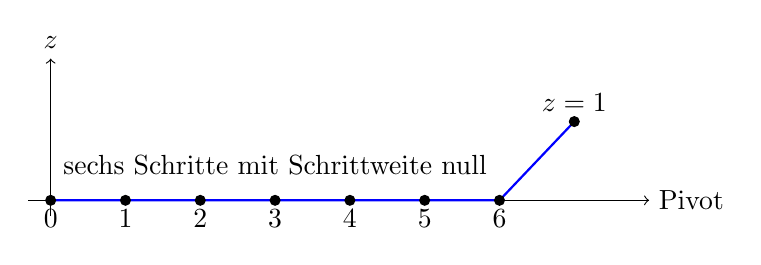
\begin{tikzpicture}[x=0.95cm,y=1cm]
\draw[->] (-0.3,0)--(8,0) node[right]{Pivot};
\draw[->] (0,-0.2)--(0,1.8) node[above]{$z$};
\draw[thick,blue] (0,0)--(6,0)--(7,1);
\foreach \x in {0,...,6}{\fill (\x,0) circle (2pt);\node[below] at (\x,0){\x};}
\fill (7,1) circle (2pt);\node[above] at (7,1){$z=1$};
\node[above] at (3,0.2){sechs Schritte mit Schrittweite null};
\end{tikzpicture}}
\aufgabe{Exercise 7.2 (On weak duality)}
\angabe{Consider the LP
\[
\max\; x_1 + 2x_2 + x_3 + 3x_4 \quad \text{s.t.}\quad
x_1 + 2x_2 + x_3 = 4,\quad x_2 + 2x_3 + x_4 = 4,\quad x_1 + x_3 + 2x_4 = 4,\quad x \ge 0.
\]
1. Determine $A$, $b$, $c$. 2. Determine the dual problem. 3. Find three feasible points each for the primal and the dual problem, compute the objective value in each case, and verify weak duality.}

\teil{Part 1: the data}
Matching the standard form $\max c^Tx$ s.t. $Ax=b$, $x\ge 0$:
\[
A = \begin{pmatrix}1&2&1&0\\0&1&2&1\\1&0&1&2\end{pmatrix},\qquad b = \begin{pmatrix}4\\4\\4\end{pmatrix},\qquad c = \begin{pmatrix}1\\2\\1\\3\end{pmatrix}.
\]

\teil{Part 2: the dual}
By Definition 3.1 the dual of $\max c^Tx$ s.t. $Ax=b$, $x\ge0$ is $\min b^Ty$ s.t. $A^Ty\ge c$, $y$ free. With
\[
A^T = \begin{pmatrix}1&0&1\\2&1&0\\1&2&1\\0&1&2\end{pmatrix}
\]
the dual reads
\begin{align*}
\min\;& 4y_1 + 4y_2 + 4y_3\\
\text{s.t.}\;& y_1 + y_3 \ge 1 && \why{column 1 of $A$, dual constraint for $x_1$}\\
& 2y_1 + y_2 \ge 2 && \why{column 2 of $A$, dual constraint for $x_2$}\\
& y_1 + 2y_2 + y_3 \ge 1 && \why{column 3 of $A$, dual constraint for $x_3$}\\
& y_2 + 2y_3 \ge 3 && \why{column 4 of $A$, dual constraint for $x_4$}\\
& y_1, y_2, y_3 \text{ free} && \why{primal constraints are equalities}
\end{align*}
\explain{Die Dualisierung tauscht die Rollen: Jede der drei primalen Gleichungen erzeugt eine freie duale Variable $y_i$, jede der vier primalen Variablen erzeugt eine duale Ungleichung (Spalte von $A$ transponiert). Die rechte Seite $b$ wird zur dualen Zielfunktion, der Kostenvektor $c$ zur rechten Seite der dualen Ungleichungen.}

\teil{Part 3: feasible points and weak duality}
For $x^{(1)}=(1,1,1,1)^T$, every component is nonnegative. Check each equation and the objective:
\begin{align*}
(Ax^{(1)})_1 &= 1\cdot 1 + 2\cdot 1 + 1\cdot 1 + 0\cdot 1 && \why{substitute the point}\\
&= 1 + 2 + 1 + 0 && \why{multiply}\\
&= 4 && \why{add}\\
(Ax^{(1)})_2 &= 0\cdot 1 + 1\cdot 1 + 2\cdot 1 + 1\cdot 1 && \why{substitute the point}\\
&= 0 + 1 + 2 + 1 && \why{multiply}\\
&= 4 && \why{add}\\
(Ax^{(1)})_3 &= 1\cdot 1 + 0\cdot 1 + 1\cdot 1 + 2\cdot 1 && \why{substitute the point}\\
&= 1 + 0 + 1 + 2 && \why{multiply}\\
&= 4 && \why{add}\\
c^Tx^{(1)} &= 1\cdot 1 + 2\cdot 1 + 1\cdot 1 + 3\cdot 1 && \why{substitute into the objective}\\
&= 1 + 2 + 1 + 3 && \why{multiply}\\
&= 7 && \why{add}
\end{align*}
\[\boxed{Ax^{(1)}=b,\quad c^Tx^{(1)}=7}\]
\explain{Jede Zeile muss genau die rechte Seite $4$ treffen. Nichtnegativität allein reicht für die primale Zulässigkeit nicht. Erst nach dieser Probe berechnen wir den Zielfunktionswert.}
For $x^{(2)}=(0,2,0,2)^T$, every component is nonnegative. Check each equation and the objective:
\begin{align*}
(Ax^{(2)})_1 &= 1\cdot 0 + 2\cdot 2 + 1\cdot 0 + 0\cdot 2 && \why{substitute the point}\\
&= 0 + 4 + 0 + 0 && \why{multiply}\\
&= 4 && \why{add}\\
(Ax^{(2)})_2 &= 0\cdot 0 + 1\cdot 2 + 2\cdot 0 + 1\cdot 2 && \why{substitute the point}\\
&= 0 + 2 + 0 + 2 && \why{multiply}\\
&= 4 && \why{add}\\
(Ax^{(2)})_3 &= 1\cdot 0 + 0\cdot 2 + 1\cdot 0 + 2\cdot 2 && \why{substitute the point}\\
&= 0 + 0 + 0 + 4 && \why{multiply}\\
&= 4 && \why{add}\\
c^Tx^{(2)} &= 1\cdot 0 + 2\cdot 2 + 1\cdot 0 + 3\cdot 2 && \why{substitute into the objective}\\
&= 0 + 4 + 0 + 6 && \why{multiply}\\
&= 10 && \why{add}
\end{align*}
\[\boxed{Ax^{(2)}=b,\quad c^Tx^{(2)}=10}\]
\explain{Jede Zeile muss genau die rechte Seite $4$ treffen. Nichtnegativität allein reicht für die primale Zulässigkeit nicht. Erst nach dieser Probe berechnen wir den Zielfunktionswert.}
For $x^{(3)}=(2,0,2,0)^T$, every component is nonnegative. Check each equation and the objective:
\begin{align*}
(Ax^{(3)})_1 &= 1\cdot 2 + 2\cdot 0 + 1\cdot 2 + 0\cdot 0 && \why{substitute the point}\\
&= 2 + 0 + 2 + 0 && \why{multiply}\\
&= 4 && \why{add}\\
(Ax^{(3)})_2 &= 0\cdot 2 + 1\cdot 0 + 2\cdot 2 + 1\cdot 0 && \why{substitute the point}\\
&= 0 + 0 + 4 + 0 && \why{multiply}\\
&= 4 && \why{add}\\
(Ax^{(3)})_3 &= 1\cdot 2 + 0\cdot 0 + 1\cdot 2 + 2\cdot 0 && \why{substitute the point}\\
&= 2 + 0 + 2 + 0 && \why{multiply}\\
&= 4 && \why{add}\\
c^Tx^{(3)} &= 1\cdot 2 + 2\cdot 0 + 1\cdot 2 + 3\cdot 0 && \why{substitute into the objective}\\
&= 2 + 0 + 2 + 0 && \why{multiply}\\
&= 4 && \why{add}
\end{align*}
\[\boxed{Ax^{(3)}=b,\quad c^Tx^{(3)}=4}\]
\explain{Jede Zeile muss genau die rechte Seite $4$ treffen. Nichtnegativität allein reicht für die primale Zulässigkeit nicht. Erst nach dieser Probe berechnen wir den Zielfunktionswert.}
For $y^{(1)}=(1,1,1)^T$, the variables may have either sign:
\begin{align*}
(A^Ty^{(1)})_{1} &= 1\cdot 1 + 0\cdot 1 + 1\cdot 1 && \why{substitute into the dual constraint}\\
&= 1 + 0 + 1 && \why{multiply}\\
&= 2 && \why{add}\\
2 &\ge 1 && \why{compare with the component of $c$}\\
(A^Ty^{(1)})_{2} &= 2\cdot 1 + 1\cdot 1 + 0\cdot 1 && \why{substitute into the dual constraint}\\
&= 2 + 1 + 0 && \why{multiply}\\
&= 3 && \why{add}\\
3 &\ge 2 && \why{compare with the component of $c$}\\
(A^Ty^{(1)})_{3} &= 1\cdot 1 + 2\cdot 1 + 1\cdot 1 && \why{substitute into the dual constraint}\\
&= 1 + 2 + 1 && \why{multiply}\\
&= 4 && \why{add}\\
4 &\ge 1 && \why{compare with the component of $c$}\\
(A^Ty^{(1)})_{4} &= 0\cdot 1 + 1\cdot 1 + 2\cdot 1 && \why{substitute into the dual constraint}\\
&= 0 + 1 + 2 && \why{multiply}\\
&= 3 && \why{add}\\
3 &\ge 3 && \why{compare with the component of $c$}\\
b^Ty^{(1)} &= 4\cdot 1 + 4\cdot 1 + 4\cdot 1 && \why{substitute into the objective}\\
&= 4 + 4 + 4 && \why{multiply}\\
&= 12 && \why{add}
\end{align*}
\[\boxed{A^Ty^{(1)}\ge c,\quad b^Ty^{(1)}=12}\]
\explain{Beim dualen Punkt prüfen wir jede Ungleichung. Die linke Seite darf größer als die entsprechende Komponente von $c$ sein; Gleichheit ist nicht verlangt.}
For $y^{(2)}=(1,3,0)^T$, the variables may have either sign:
\begin{align*}
(A^Ty^{(2)})_{1} &= 1\cdot 1 + 0\cdot 3 + 1\cdot 0 && \why{substitute into the dual constraint}\\
&= 1 + 0 + 0 && \why{multiply}\\
&= 1 && \why{add}\\
1 &\ge 1 && \why{compare with the component of $c$}\\
(A^Ty^{(2)})_{2} &= 2\cdot 1 + 1\cdot 3 + 0\cdot 0 && \why{substitute into the dual constraint}\\
&= 2 + 3 + 0 && \why{multiply}\\
&= 5 && \why{add}\\
5 &\ge 2 && \why{compare with the component of $c$}\\
(A^Ty^{(2)})_{3} &= 1\cdot 1 + 2\cdot 3 + 1\cdot 0 && \why{substitute into the dual constraint}\\
&= 1 + 6 + 0 && \why{multiply}\\
&= 7 && \why{add}\\
7 &\ge 1 && \why{compare with the component of $c$}\\
(A^Ty^{(2)})_{4} &= 0\cdot 1 + 1\cdot 3 + 2\cdot 0 && \why{substitute into the dual constraint}\\
&= 0 + 3 + 0 && \why{multiply}\\
&= 3 && \why{add}\\
3 &\ge 3 && \why{compare with the component of $c$}\\
b^Ty^{(2)} &= 4\cdot 1 + 4\cdot 3 + 4\cdot 0 && \why{substitute into the objective}\\
&= 4 + 12 + 0 && \why{multiply}\\
&= 16 && \why{add}
\end{align*}
\[\boxed{A^Ty^{(2)}\ge c,\quad b^Ty^{(2)}=16}\]
\explain{Beim dualen Punkt prüfen wir jede Ungleichung. Die linke Seite darf größer als die entsprechende Komponente von $c$ sein; Gleichheit ist nicht verlangt.}
For $y^{(3)}=(0,3,1)^T$, the variables may have either sign:
\begin{align*}
(A^Ty^{(3)})_{1} &= 1\cdot 0 + 0\cdot 3 + 1\cdot 1 && \why{substitute into the dual constraint}\\
&= 0 + 0 + 1 && \why{multiply}\\
&= 1 && \why{add}\\
1 &\ge 1 && \why{compare with the component of $c$}\\
(A^Ty^{(3)})_{2} &= 2\cdot 0 + 1\cdot 3 + 0\cdot 1 && \why{substitute into the dual constraint}\\
&= 0 + 3 + 0 && \why{multiply}\\
&= 3 && \why{add}\\
3 &\ge 2 && \why{compare with the component of $c$}\\
(A^Ty^{(3)})_{3} &= 1\cdot 0 + 2\cdot 3 + 1\cdot 1 && \why{substitute into the dual constraint}\\
&= 0 + 6 + 1 && \why{multiply}\\
&= 7 && \why{add}\\
7 &\ge 1 && \why{compare with the component of $c$}\\
(A^Ty^{(3)})_{4} &= 0\cdot 0 + 1\cdot 3 + 2\cdot 1 && \why{substitute into the dual constraint}\\
&= 0 + 3 + 2 && \why{multiply}\\
&= 5 && \why{add}\\
5 &\ge 3 && \why{compare with the component of $c$}\\
b^Ty^{(3)} &= 4\cdot 0 + 4\cdot 3 + 4\cdot 1 && \why{substitute into the objective}\\
&= 0 + 12 + 4 && \why{multiply}\\
&= 16 && \why{add}
\end{align*}
\[\boxed{A^Ty^{(3)}\ge c,\quad b^Ty^{(3)}=16}\]
\explain{Beim dualen Punkt prüfen wir jede Ungleichung. Die linke Seite darf größer als die entsprechende Komponente von $c$ sein; Gleichheit ist nicht verlangt.}
All nine feasible pairs satisfy weak duality:
\begin{align*}
7 &\le 12 && \why{pair $(x^{(1)},y^{(1)})$}\\
7 &\le 16 && \why{pair $(x^{(1)},y^{(2)})$}\\
7 &\le 16 && \why{pair $(x^{(1)},y^{(3)})$}\\
10 &\le 12 && \why{pair $(x^{(2)},y^{(1)})$}\\
10 &\le 16 && \why{pair $(x^{(2)},y^{(2)})$}\\
10 &\le 16 && \why{pair $(x^{(2)},y^{(3)})$}\\
4 &\le 12 && \why{pair $(x^{(3)},y^{(1)})$}\\
4 &\le 16 && \why{pair $(x^{(3)},y^{(2)})$}\\
4 &\le 16 && \why{pair $(x^{(3)},y^{(3)})$}
\end{align*}
\[\boxed{c^Tx^{(i)}\le b^Ty^{(j)}\quad (i,j\in\{1,2,3\})}\]
\explain{Wie man die primalen Punkte findet: Jede Zeile von $A$ hat die Zeilensumme $4$ gleich der rechten Seite. Kombinationen aus $0,1,2$ mit den passenden Spalten treffen diese Summe. $(1,1,1,1)$ addiert in jeder Zeile alle drei von null verschiedenen Koeffizienten. Bei $(0,2,0,2)$ und $(2,0,2,0)$ werden dagegen nur die jeweils ausgewählten Spalten mit $2$ multipliziert. Bei den dualen Punkten prüft man die vier Ungleichungen einzeln; keine der vier Prüfungen darf ausgelassen werden.}
\explain{$(0,2,0,2)$ hat den Zielfunktionswert $10$, der kleinste duale Wert hier ist $12$. Die Lücke $12-10=2$ ist nur ein Abstand zwischen den gewählten Punkten, keine Dualitätslücke: Nach starker Dualität ist der wahre optimale Wert $10$, erreicht etwa von $y^*=(\tfrac74,-\tfrac32,\tfrac94)$ mit $b^Ty^*=10$. Die schwache Dualität verlangt nur, dass kein primaler Wert einen dualen übertrifft.}

\aufgabe{Exercise 7.3 (On strong duality)}
\angabe{Show that strong duality as stated in Theorem 3.7 and the corresponding proof imply: If (P) has an optimal solution, so does (D) and $\nu_P = \nu_D$. Hint: Use the same arguments as in the proof of Theorem 3.7 to show that (D) is feasible.}

\teil{Setup}
Let (P) have an optimal solution. Then it is feasible and bounded above. First assume $\operatorname{rank}(A)=m$. Start at a feasible basis and run simplex with Bland's rule. Bland's rule prevents cycling, so the run terminates. It cannot terminate with an unboundedness certificate, since (P) has a finite optimum. It therefore reaches a feasible dictionary with all reduced costs nonpositive. Denote its basic solution by $x^*$, its basis by $B$ and its nonbasis by $N$. This choice matters: an arbitrary basis representing an optimal degenerate point need not have nonpositive reduced costs. The terminating dictionary is
\begin{align*}
x_B &= A_B^{-1}b - A_B^{-1}A_Nx_N && \why{split $Ax=b$ at the basis $B$}\\
z &= c_B^TA_B^{-1}b + (c_N^T - c_B^TA_B^{-1}A_N)x_N && \why{express the objective in $x_N$}
\end{align*}

\teil{The dual candidate}
Define
\begin{align*}
y^{*T} &:= c_B^TA_B^{-1}
\end{align*}
For the basic columns this gives equality, for the nonbasic columns optimality gives the needed inequality. For $j\in B$, write $k$ for its position in the ordered basis:
\begin{align*}
y^{*T}A_j &= c_B^TA_B^{-1}A_j && \why{definition of $y^*$}\\
&= c_B^Te_k && \why{$k$ is the position of column $j$ in $B$}\\
&= c_j && \why{unit vector selects that cost}
\end{align*}
For $j\in N$, the reduced cost is nonpositive at an optimal dictionary of a maximization problem:
\begin{align*}
c_j - c_B^TA_B^{-1}A_j &\le 0 && \why{optimality condition, reduced cost of $x_j$}\\
c_j &\le c_B^TA_B^{-1}A_j && \why{add $c_B^TA_B^{-1}A_j$}\\
c_j &\le y^{*T}A_j && \why{definition of $y^*$}
\end{align*}
Together these two cases give $A^Ty^* \ge c$, that is, $y^*$ is feasible for (D).
\explain{Das ist der Kern: Die negativen reduzierten Kosten sind die Schlupfwerte der dualen Ungleichungen. Für eine Nichtbasisvariable gilt also $A_j^Ty^*-c_j=-\bar c_j\ge0$. Der Vektor $y^{*T}=c_B^TA_B^{-1}$ (die Simplex-Multiplikatoren) wird aus der optimalen Basis abgelesen und erfüllt $A^Ty^*\ge c$ komponentenweise: für Basisindizes mit Gleichheit, für Nichtbasisindizes wegen der Optimalität.}

\teil{Equal objective values}
The dual objective at $y^*$ equals the primal optimum:
\begin{align*}
b^Ty^* &= b^T(A_B^{-1})^Tc_B && \why{transpose the definition: $y^* = (A_B^{-1})^Tc_B$}\\
&= (A_B^{-1}b)^Tc_B && \why{move the transpose}\\
&= (x^*_B)^Tc_B && \why{$x^*_B = A_B^{-1}b$ at the basic feasible solution}\\
&= c_B^Tx^*_B && \why{scalar transpose}\\
&= c^Tx^* && \why{$x^*_N = 0$, so $c^Tx^* = c_B^Tx^*_B$}\\
&= \nu_P && \why{definition of the optimal value}
\end{align*}

\teil{Optimality via weak duality}
For every dual feasible $\tilde y$, weak duality (Theorem 3.3) gives
\begin{align*}
c^Tx^* &\le b^T\tilde y && \why{$x^*$ primal feasible, $\tilde y$ dual feasible}\\
\nu_P &\le b^T\tilde y && \why{$c^Tx^* = \nu_P$}
\end{align*}
Every dual feasible point has value at least $\nu_P$. Since $y^*$ is dual feasible with $b^Ty^* = \nu_P$, it attains this lower bound:
\begin{align*}
b^Ty^* &\le b^T\tilde y && \why{$\tilde y$ arbitrary, $b^Ty^* = \nu_P \le b^T\tilde y$}
\end{align*}
Hence $y^*$ minimizes $b^Ty$ over the dual feasible set, so $y^*$ is an optimal solution of (D) and
\[
\boxed{\nu_D = b^Ty^* = \nu_P}
\]
\teil{Dependent equality rows}
If $A$ has dependent rows, choose independent rows $A_I$ spanning its row space. Since (P) is feasible, every dependence among rows of $A$ also holds for the corresponding entries of $b$. Thus deleting the other equalities leaves the feasible set and objective unchanged. Apply the full-row-rank construction to $(A_I,b_I,c)$ and obtain $y_I^*$. Set $y_i^*=0$ for each deleted row. Then
\begin{align*}
A^Ty^* &= A_I^Ty_I^* && \why{deleted coordinates of $y^*$ are zero}\\
A_I^Ty_I^* &\ge c && \why{dual feasibility in the reduced system}\\
b^Ty^* &= b_I^Ty_I^* && \why{deleted coordinates contribute zero}\\
&= \nu_P && \why{reduced primal has the same optimum}
\end{align*}
Weak duality again proves that this lifted vector is dual optimal. If $\operatorname{rank}(A)=0$, primal feasibility forces $b=0$. Boundedness forces $c\le0$, since any positive cost could be increased along its coordinate axis. The vector $y^*=0$ is then dual feasible and both optima are zero.
\[\boxed{\text{(P) has an optimum }\Longrightarrow\text{ (D) has an optimum and }\nu_P=\nu_D.}\qquad\square\]
\explain{Abhängige Gleichungen schränken die zulässigen Punkte nicht weiter ein. Wir entfernen sie für die Rechnung und setzen ihre dualen Variablen danach auf null. Dadurch bleiben sowohl $A^Ty$ als auch der duale Zielfunktionswert so, wie sie im reduzierten System waren.}
\explain{Der Schluss ist ein Sandwich: Schwache Dualität sagt $c^Tx\le b^Ty$ für jedes zulässige Paar. Weil das konstruierte $y^*$ den Wert exakt $b^Ty^*=\nu_P$ trifft, kann kein dualer Punkt darunter liegen, sonst würde er die schwache Dualität verletzen. Also ist $y^*$ dual optimal, und beide Optimalwerte stimmen überein.}
\explain{Warum reicht es laut Hinweis, die Zulässigkeit von (D) zu zeigen? Sobald $y^*$ dual zulässig ist und $b^Ty^*=\nu_P$ gilt, erledigt die schwache Dualität den Rest automatisch: Sie liefert $\nu_P\le b^Ty$ für alle dual zulässigen $y$ und damit die Optimalität von $y^*$. Die Existenz einer dualen Optimallösung folgt also nicht aus einer separaten Annahme, sondern aus der explizit hingeschriebenen Lösung $y^{*T}=c_B^TA_B^{-1}$.}

\end{document}
